We show in the following proposition how the mode-$n$ product can be expressed through matricization and matrix product. 
\begin{proposition}
Let $\Xt\in\RR^{d_1\times\dots\times d_N}$ and $\Mb\in\RR^{m\times d_n}$ then 
$(\Xt\ttm n \Mb)_{(n)} = \Mb\Xt_{(n)}$.
\begin{proof}
We show this identity with a simple tensor network diagram for the special case $n=2$ and $N=3$. The extension to the general case is straightforward. We have
\begin{align*}
(\Xt\ttm2\Mb)_{(2)} 
&= 
\left(
    \begin{tikzpicture}[baseline=\baseline]
    \tikzset{tensor/.style = {minimum size = 0.5cm,shape = circle,thick,draw=black,inner sep = 0pt}, edge/.style = {thick,line width=.4mm},every loop/.style={}}
    \def\y{0}
    \def\x{0}
    \node[tensor,fill=green!50!red!50!white] (At) at (\x,\y){\scalebox{0.85}{$\Xt$}};
    \node[tensor,fill=blue!20!white] (M) at (\x-1,\y) {$\Mb$};
    \draw[edge] (At) -- (M) node [midway,above]
    {\scalebox{0.7}{\dimcolor{$d_2$}}};
    \draw[edge] (M) -- (\x-1.7,\y) node [midway,above]
    {\scalebox{0.7}{\dimcolor{$m$}}};);
    \draw[edge] (At)-- (\x+0.5,\y+0.5) node [below] {\scalebox{0.7}{\dimcolor{$d_1$}}};
    \draw[edge] (At)-- (\x+0.5,\y-0.5) node [above] {\scalebox{0.7}{\dimcolor{$d_3$}}};
    \end{tikzpicture}
\right)_{(2)}
=
    \begin{tikzpicture}[baseline=\baseline]
    \tikzset{tensor/.style = {minimum size = 0.5cm,shape = circle,thick,draw=black,inner sep = 0pt}, edge/.style = {thick,line width=.4mm},every loop/.style={}}
    \def\y{0}
    \def\x{0}
    \node[tensor,fill=green!50!red!50!white] (At) at (\x,\y){\scalebox{0.85}{$\Xt$}};
    \node[tensor,fill=blue!20!white] (M) at (\x-1,\y) {$\Mb$};
    \draw[edge] (At) -- (M) node [midway,above]
    {\scalebox{0.7}{\dimcolor{$d_2$}}};
    \draw[edge] (M) -- (\x-1.7,\y) node [midway,above]
    {\scalebox{0.7}{\dimcolor{$m$}}};);
    \draw[edge] (\x+0.15,\y+0.2)-- (\x+0.5,\y+0.2)-- (\x+0.5,\y+0.05) -- (\x+1,\y+0.05) node [above] {\scalebox{0.7}{\dimcolor{$d_1$}}};
    \draw[edge] (\x+0.15,\y-0.2) -- (\x+0.5,\y-0.2)--(\x+0.5,\y-0.04)--(\x+1,\y-0.04) node [below] {\scalebox{0.7}{\dimcolor{$d_3$}}};
    \end{tikzpicture}\\
&=
\Mb\Xt_{(2)} \in\RR^{m\times d_1d_3}.
\end{align*}
\end{proof}
\end{proposition}
\item\textbf{Mode-n product~(vector).} The mode-$n$ product of a tensor $\Xt\in\RR^{d_1\times\cdots\times d_N}$ with a vector $\vb\in\RR^{d_n}$, is denoted by 
$\Xt \ttm n \vb \in\RR^{d_1\times\cdots \times d_{n-1}\times d_{n+1}\times \cdots\times d_N}$. Note that the result is a tensor of order $N-1$. It can be pictured in a tensor network diagram as 
    $$
\Xt\ttm n \vb
=
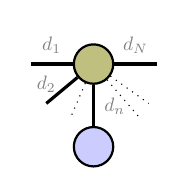
\begin{tikzpicture}[baseline=-0.5ex]
    \tikzset{tensor/.style = {minimum size = 0.5cm,shape = circle,thick,draw=black,inner sep = 0pt}, edge/.style = {thick,line width=.4mm},every loop/.style={}}
    \def\x{6}
    \node[tensor,fill=blue!20!white] (M) at (\x,-1.05) {$\vb$};
    \node[tensor,fill=green!50!red!50!white] (At) at 
    (\x,0) {$\Xt$};
    \draw[edge] (At) -- (\x-0.8,0) node [midway,above] {\scalebox{0.7}{\textcolor{gray}{$d_1$}}};
    \draw[edge] (At)-- (\x-0.6,-0.5) node [above]{\scalebox{0.7}{\textcolor{gray}{$d_2$}}};
    \draw[edge] (At) -- (\x+0.8,0) node [midway,above] {\scalebox{0.7}{\textcolor{gray}{$d_N$}}};;
    \draw[dotted] (At) -- (\x-0.3,-0.7);
    \draw[edge] (At) -- (\x,-0.8) node [midway,right] {\scalebox{0.7}{\textcolor{gray}{$d_n$}}};
    \draw[dotted] (At) -- (\x+0.6,-0.7);
    \draw[dotted] (At) -- (\x+0.7,-0.5);
    \end{tikzpicture}
\in\RR^{d_1\times  \dots\times d_{n-1}\times d_{n+1}\times \dots\times d_N}.
$$
Note that in mode-$n$ vector multiplication, unlike mode-$n$ matrix multiplication, the order of multiplication matters as a vector contraction reduces the tensor order by 1, so subsequent mode indices shift. Let $\Xt\in\RR^{d_1\times\cdots\times d_m\times\cdots\times d_n\times\cdots\times d_N}$ and $\ab\in\RR^{d_n},\bb\in\RR^{d_m}$, then
$
\Xt\ttm n \ab\ttm m\bb \neq
(\Xt \ttm m \bb)\ttm{n}\ab,
$
as mode-$n$ vector multiplication drops the $m$-th dimension~\citep{bader2006algorithm}.
\end{enumerate}







Next, we introduce several important products that are often used in tensor derivations: Kronecker, Khatri-Rao, and Hadamard products.

\paragraph{Kronecker product}\label{subsection-kron}
Let $\Ab\in\RR^{m\times n}$ and $\Bb\in\RR^{p\times q}$. The Kronecker product, $\Ab\kron\Bb\in\RR^{mp\times nq}$ is defined by
\begin{align}
    \Ab\kron\Bb = 
    \begin{bmatrix}
    a_{11}\Bb & a_{12}\Bb & \dots & a_{1n}\Bb \\
    a_{21}\Bb & a_{22}\Bb & \dots & a_{2n}\Bb \\
    \vdots & \vdots & \ddots & \vdots \\
    a_{m1}\Bb & a_{m2}\Bb & \dots & a_{mn}\Bb 
    \end{bmatrix}.
\end{align}

In tensor networks, the Kronecker product is given by the following diagram:
\begin{align}
    \Ab\kron\Bb = 
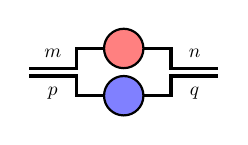
\begin{tikzpicture}[baseline=-0.5ex]
    \tikzset{tensor/.style = {minimum size = 0.5cm,shape = circle,thick,draw=black,inner sep = 0pt}, edge/.style   = {thick,line width=.4mm}}
    \def\x{0}
    \def\y{0}
    \node[tensor,fill=red!50!white] (A) at (\x,\y+0.3){$\Ab$};
    \node[tensor,fill=blue!50!white] (B) at (\x,\y-0.3){$\Bb$};
    \draw[edge] (\x-0.25,\y+0.3) -- (\x-0.6,\y+0.3) -- (\x-0.6,\y+0.05)   -- (\x-1.2,\y+0.05) node [midway,above] {\scalebox{0.7}{\dimcolor{$m$}}};
    \draw[edge] (\x-0.25,\y-0.3) -- (\x-0.6,\y-0.3) -- (\x-0.6,\y-0.05) -- (\x-1.2,\y-0.05) node [midway,below] {\scalebox{0.7}{\dimcolor{$p$}}};
    \draw[edge] (\x+0.25,\y+0.3) -- (\x+0.6,\y+0.3) -- (\x+0.6,\y+0.05) -- (\x+1.2,\y+0.05) node [midway,above] {\scalebox{0.7}{\dimcolor{$n$}}};
    \draw[edge] (\x+0.25,\y-0.3) -- (\x+0.6,\y-0.3) -- (\x+0.6,\y-0.05) -- (\x+1.2,\y-0.05) node [midway,below] {\scalebox{0.7}{\dimcolor{$q$}}};
\end{tikzpicture}.
\end{align}
As one can see from this diagram, the Kronecker product of two matrices is nothing else than a reshaping of their outer products. Indeed, it is easy to convince oneself that every component $a_{i,j}b_{k,l}$ of the outer product $\Ab \outprod \Bb$ is present in $\Ab \kron \Bb$; while the outer product is a fourth-order tensor, the Kronecker product is one of its matricizations. One could show more precisely that $\Ab \kron \Bb = (\Ab \outprod \Bb)_{(\{1,3\})}$, but we will refrain from doing so and trust the simpler and direct view given by tensor network diagrams: grouping the row legs of $\Ab$ and $\Bb$ on one side, and their column legs on the other,  we obtain the matrix called the Kronecker product of $\Ab$ and $\Bb$:
$$\Ab\outprod \Bb =    
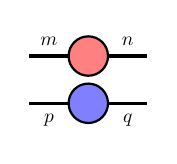
\begin{tikzpicture}[baseline=-0.5ex]
    \tikzset{tensor/.style = {minimum size = 0.5cm,shape = circle,thick,draw=black,inner sep = 0pt}, edge/.style   = {thick,line width=.4mm}}
    \def\x{0}
    \def\y{0}
    \node[tensor,fill=red!50!white] (A) at (\x,\y+0.3){$\Ab$};
    \node[tensor,fill=blue!50!white] (B) at (\x,\y-0.3){$\Bb$};
    \draw[edge] (\x-0.25,\y+0.3) -- (\x-0.75,\y+0.3) node [midway,above] {\scalebox{0.7}{\dimcolor{$m$}}};
    \draw[edge] (\x-0.25,\y-0.3) -- (\x-0.75,\y-0.3) node [midway,below] {\scalebox{0.7}{\dimcolor{$p$}}};
    \draw[edge] (\x+0.25,\y+0.3) -- (\x+0.75,\y+0.3) node [midway,above] {\scalebox{0.7}{\dimcolor{$n$}}};
    \draw[edge] (\x+0.25,\y-0.3) -- (\x+0.75,\y-0.3) node [midway,below] {\scalebox{0.7}{\dimcolor{$q$}}};
\end{tikzpicture}
\longrightarrow
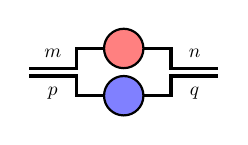
\begin{tikzpicture}[baseline=-0.5ex]
    \tikzset{tensor/.style = {minimum size = 0.5cm,shape = circle,thick,draw=black,inner sep = 0pt}, edge/.style   = {thick,line width=.4mm}}
    \def\x{0}
    \def\y{0}
    \node[tensor,fill=red!50!white] (A) at (\x,\y+0.3){$\Ab$};
    \node[tensor,fill=blue!50!white] (B) at (\x,\y-0.3){$\Bb$};
    \draw[edge] (\x-0.25,\y+0.3) -- (\x-0.6,\y+0.3) -- (\x-0.6,\y+0.05)   -- (\x-1.2,\y+0.05) node [midway,above] {\scalebox{0.7}{\dimcolor{$m$}}};
    \draw[edge] (\x-0.25,\y-0.3) -- (\x-0.6,\y-0.3) -- (\x-0.6,\y-0.05) -- (\x-1.2,\y-0.05) node [midway,below] {\scalebox{0.7}{\dimcolor{$p$}}};
    \draw[edge] (\x+0.25,\y+0.3) -- (\x+0.6,\y+0.3) -- (\x+0.6,\y+0.05) -- (\x+1.2,\y+0.05) node [midway,above] {\scalebox{0.7}{\dimcolor{$n$}}};
    \draw[edge] (\x+0.25,\y-0.3) -- (\x+0.6,\y-0.3) -- (\x+0.6,\y-0.05) -- (\x+1.2,\y-0.05) node [midway,below] {\scalebox{0.7}{\dimcolor{$q$}}};
\end{tikzpicture}
=\Ab \kron \Bb.
$$

